\section{Multiple Synthetic Risky Assets}
In this section we present an application of the learning algorithms considered above to a multi-asset allocation problem. Given the difficulties of learning a profitable strategy for historical data, we consider once again synthetic price series that can be traded profitably. To define the generative model, we start from a continuous-time formulation and then derive a discrete-time model using standard discretization techniques. In particular, we assume that the market consists of two risky asset $\{S_t^1, S_t^2\}$, whose prices evolve according to the following dynamics
\begin{equation}
	\begin{cases}
		\frac{dS_t^1}{S_t^1} &= \sigma_1 dW_t^1\\ 
		\frac{dS_t^2}{S_t^2} &= \frac{1}{2} \sigma_\chi^2 dt + \sigma_2 dW_t^2 + d\chi_t\\
		d\chi_t &= -\lambda \chi_t dt + \sigma_\chi dW_t^\chi\\
	\end{cases}
\end{equation}
where $\{W_t^1, W_t^2, W_t^\chi\}$ are standard Brownian motions such that $\E {dW_t^1 dW_t^2} = \rho dt$, with $-1 \leq \rho \leq 1$, $W_t^\chi \independent (W_t^1, W_t^2)$, 
$\sigma_1$, $\sigma_2$, $\sigma_\chi$, $\lambda >0$ and $\chi_0 = 0$. The Ornstein-Uhlenbeck process $\chi_t$ represents a mean-reverting spread between the two risky assets. Let $\widetilde{S}_t^i = \log S_t^i$, $i \in \{1,2\}$ denote the log-price. A simple application of Itô's lemma yields 
\begin{equation}
	\label{eq:sde}
	\begin{cases}
		d\widetilde{S}_t^1 &= -\frac{1}{2} \sigma_1^2 dt + \sigma_1 dW_t^1\\ 
		d\widetilde{S}_t^2 &= -\frac{1}{2} \sigma_2^2 dt + \sigma_2 dW_t^2 + d\chi_t\\
		d(e^{\lambda t} \chi_t) &= \sigma_\chi e^{\lambda t} dW_t^\chi\\
	\end{cases}
\end{equation}
Integrating between $0$ and $t$ and rearranging the various terms, we obtain
\begin{equation}
	\label{eq:sol_sde}
	\begin{cases}
		S_t^1 &= S_0^1 e^{-\frac{1}{2} \sigma_1^2 t + \sigma_1 W_t^1}\\ 
		S_t^2 &= S_0^2 e^{-\frac{1}{2} \sigma_2^2 t + \sigma_2 W_t^2 + \chi_t}\\
		\chi_t &= \sigma_\chi \int_0^t e^{-\lambda (t-u)} dW_u^\chi\\
	\end{cases}
\end{equation}
We notice that the spread is a Gaussian process and $\forall t > 0$
\begin{equation} 
	\chi_t \sim \calN\left(0, \frac{\sigma_\chi^2}{2\lambda}\left(1-e^{-2\lambda t}\right) \right)
\end{equation}
To better understand the role of the spread, let us remind that $W_t^2$ can be decomposed in the following way 
\begin{equation}
	W_t^2 = \rho W_t^1 + \sqrt{1-\rho^2} W_t^{\independent}
\end{equation}
where $W_t^{\independent} \independent W_t^1$ is a standard Brownian motion. Thus, we have 
\begin{equation}
	\frac{S_t^2}{S_t^1} = \frac{S_0^2}{S_0^1} e^{-\frac{1}{2}(\sigma_2^2 - \sigma_1^2) t + (\rho \sigma_2 - \sigma_1) W_t^1 + \sigma_2 \sqrt{1-\rho^2} W_t^{\independent}} e^{\chi_t} 
\end{equation} 
Taking the expected value, we obtain 
\begin{equation}
	\E{\frac{S_t^2}{S_t^1}} = \frac{S_0^2}{S_0^1} e^{\sigma_1 (\sigma_1 - \rho \sigma_2) t} e^{\frac{\sigma_\chi^2}{4\lambda} (1-e^{-2\lambda t})} 
\end{equation} 
The term coming from the stochastic spread disappears in the long term. In the limit case where $\sigma_1 = \sigma_2$ and $\rho = 1$. Then 
\begin{equation}
	\E{\frac{S_t^2}{S_t^1}} = \frac{S_0^2}{S_0^1} e^{\frac{\sigma_\chi^2}{4\lambda} (1-e^{-2\lambda t})} \underset{t \to \infty}{\to} \frac{S_0^2}{S_0^1}
\end{equation} 
Therefore, the expected value of the ratio between the prices of the two risky assets mean-reverts to the initial ratio. It is easy to understand that this feature can be traded profitably by betting on the convergence of the two assets to their long-term regime.\\
The solutions of the system (\ref{eq:sol_sde}) can be easily used to simulate the risky assets prices, which can then be used as inputs of the asset allocation problem. An alternative approach is to obtain the discrete-time dynamics of the system. Let us consider a uniform time-grid $t_k = k \Delta t$, $k \in \mathbb{N}$, and let us integrate the system (\ref{eq:sde}) between $t_k$ and $t_{k+1}$. After some simple algebraic manipulations, we obtain the following equations 
\begin{equation}
	\label{eq:dt_dynamics}
	\begin{cases}
		\widetilde{S}_{k+1}^1 &= \widetilde{S}_{k}^1 -\frac{1}{2} \sigma_1^2 \Delta t + \sigma_1 \sqrt{t} \epsilon_k^1\\ 
		\widetilde{S}_{k+1}^2 &= \widetilde{S}_{k}^2 -\frac{1}{2} \sigma_2^2 \Delta t + \sigma_2 \sqrt{t} \epsilon_k^2 + \chi_{k+1} - \chi_k\\
		\chi_{k+1} &= e^{-\lambda \Delta t} \chi_k + \sigma_\chi \sqrt{\frac{1-e^{-2\lambda \Delta t}}{2\lambda}} \epsilon_k^\chi
	\end{cases}
\end{equation}
where the noises are a Gaussain white noise with the following structure
\begin{equation}
	\begin{bmatrix}
	  	\epsilon_k^1\\
	  	\epsilon_k^2\\
	  	\epsilon_k^\chi\\	  
	\end{bmatrix} \sim \calN\left( 
	\begin{bmatrix}
		  	0\\
		  	0\\
		  	0\\	  
	\end{bmatrix}, 
	\begin{bmatrix}
		  	1, \rho, 0\\
		  	\rho, 1, 0\\
		  	0, 0, 1\\	  
	\end{bmatrix}	
	\right)
\end{equation}
We expect to be possible to trade the two risky assets profitably using an approach similar to the well-known pairs trading technique for cointegrated assets. Intuitively, because of the mean-reversion of the stochastic spread, we should be able to generate a profit by betting on the convergence of the prices of the two assets when they are far apart by selling the more expensive asset and buying the cheaper one. For these considerations, we expect the RL algorithms discussed in the previous chapters to be able to spot this pattern and exploit it to generate a profit. 

\begin{figure}[t!]
	\centering
	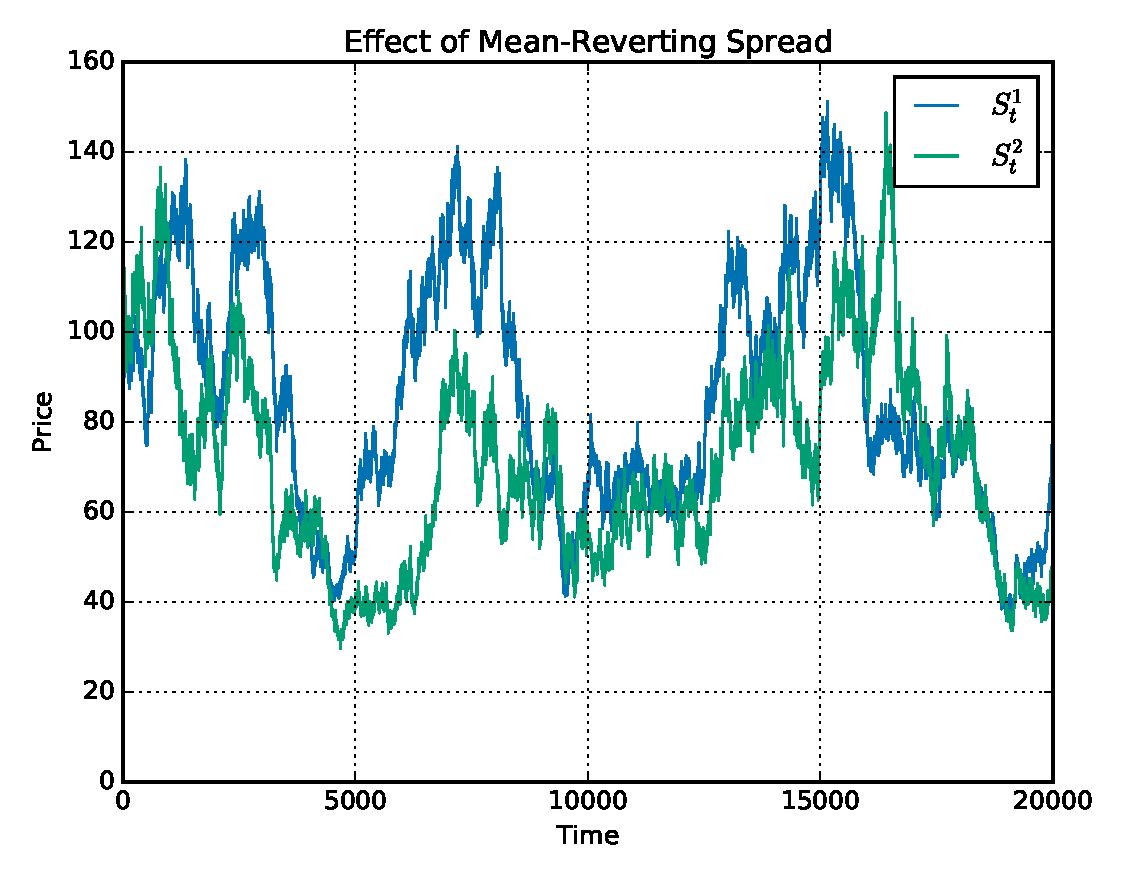
\includegraphics[width=0.8\textwidth]{Images/8_cointegrated_series}
	\caption[Sample paths for the risky assets with a mean-reverting spread.]{Sample paths for the risky assets with a mean-reverting spread.}
	\label{fig:cointegrated_series}
\end{figure}

\subsection{Specifications of the Learning Algorithms}
The parametric policies used in Section \ref{sec:synthetic_risky_asset} can be directly used in this setting to select the weight of one of the assets. Given the poor results obtained with ARAC, we only focus on the PGPE and NPGPE algorithms. The weight on the first asset is selected using The following controller 
\begin{equation*}
	a^1 = F_\theta(s) = \sign(\theta \cdot s)
\end{equation*}
where in PGPE the parameters are sampled from a multi-variate Gaussian distribution
\begin{equation*}
	\theta \sim \calN(\mu, \diag(\sigma))
\end{equation*}  
while in NPGPE the controller parameters are sampled from a Gaussian distribution parameterized by its mean and Cholesky factor
\begin{equation*}
	\theta \sim \calN(\mu, C^T C)
\end{equation*}  
The long-short strategy is completed by selecting $a^2 = - a^1$. In this case we notice that $a^1 + a^2 = 0$, which means that the long position on one asset is entirely financed by the short position on the other asset. Clearly, this assumption is simplistic as it neglects all the practical constraints on short-selling. Given that we will always be short on one of the two assets, we will also neglect short-selling fees, i.e. $\delta_s = 0$. 